\documentclass[border=1pt,tikz,svgnames]{standalone}
\usepackage{tikz}
\usetikzlibrary{decorations.markings,arrows.meta,calc}
\tikzset{>={Stealth[length=1.2mm,width=1.2mm]}} % default arrow tip for -> etc.

% 2024 Cambridge brand colours used for the curvature (Crest) and torsion
% (Cherry) panels of this figure.  Standalone preamble, so we define them
% here instead of pulling from the talk theme.
\definecolor{Cambridge24Crest}{HTML}{FD8153}
\definecolor{Cambridge24DarkCrest}{HTML}{DD3025}
\definecolor{Cambridge24Cherry}{HTML}{CD3572}
\definecolor{Cambridge24DarkCherry}{HTML}{911449}
\definecolor{Cambridge24DarkBlue}{HTML}{133844} % structural ink (CamDarkBlue)

\colorlet{OrangeFill}{Cambridge24Crest}
\colorlet{OrangeLine}{Cambridge24DarkCrest}
\colorlet{PurpleFill}{Cambridge24Cherry}
\colorlet{PurpleLine}{Cambridge24DarkCherry}
\colorlet{InkBlue}{Cambridge24DarkBlue} % neutral transport paths + R/T labels

\tikzset{
  DashedArrows/.style 2 args={
      densely dashed, thin,
      postaction={decorate},
      decoration={markings,
          mark=at position #1 with {\arrow{>}},
          mark=at position #2 with {\arrow{>}}
        }
    }
}

\begin{document}

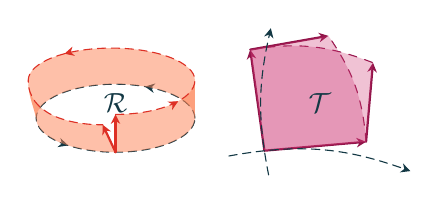
\begin{tikzpicture}[line cap=round]
  \def\Lx{1.44}
  \def\Ly{0.96}
  \begin{scope}[shift={(0,0)}]
    \def\Rx{0.7*\Lx}
    \def\Ry{0.45*\Ly}
    \coordinate (O) at (0,-0.2*\Ly);
    \draw[InkBlue, DashedArrows={0.17}{0.62}] (0,-0.2*\Ly) ellipse ({\Rx} and {\Ry});
    \fill[OrangeFill, opacity=0.5] (\Rx,0.3*\Ly) arc(0:-90:{\Rx} and {\Ry}) --++ (0,-0.5*\Ly) arc(-90:0:{\Rx} and {\Ry}) -- cycle;
    \fill[OrangeFill, opacity=0.5] (\Rx,0.3*\Ly) arc(0:180:{1.05*\Rx} and {0.95*\Ry}) -- (-1.1*\Rx,0.3*\Ly) to[out=-90,in=103] (-\Rx,-0.2*\Ly) arc(180:0:{\Rx} and {\Ry}) -- cycle;
    \fill[OrangeFill, opacity=0.5] ($(O)+(0,-\Ry)$) arc(-90:-180:{\Rx} and {\Ry}) to[out=103,in=-90] (-1.1*\Rx,0.3*\Ly) to[out=-90,in=180] ($(O)+(0,-\Ry)+(115:0.4*\Ly)$) -- cycle;

    \draw[OrangeLine, DashedArrows={0.17}{0.62}] ($(O)+(0,0.5*\Ly-\Ry)$) arc(-90:0:{\Rx} and {\Ry}) arc(0:180:{1.05*\Rx} and {0.95*\Ry}) to[out=-90,in=180] ($(O)+(0,-\Ry)+(115:0.4*\Ly)$);

    \draw[OrangeLine, thick, ->] ($(O)+(0,-\Ry)$) --++ (0,0.5*\Ly);
    \draw[OrangeLine, thick, ->] ($(O)+(0,-\Ry)$) --++ (115:0.4*\Ly);

    \node[InkBlue] at (0,0) {$\mathcal{R}$};
  \end{scope}

  \begin{scope}[shift={(1.8*\Lx,0)}]
    \coordinate (O) at (-0.487*\Lx,-0.63*\Ly);
    \coordinate (R) at ($(O)+(98:0.9*\Lx)$);
    \coordinate (Ru) at ($(O)+(98:0.9*\Lx)+(10:0.7*\Lx)$);
    \coordinate (Q) at ($(O)+(5:0.9*\Lx)$);
    \coordinate (Qv) at ($(O)+(5:0.9*\Lx)+(85:0.7*\Lx)$);

    \draw[PurpleLine, thick, ->] (O) -- (R);
    \draw[PurpleLine, thick, ->] (O) -- (Q);
    \draw[PurpleLine, thick, ->] (R) -- (Ru);
    \draw[PurpleLine, thick, ->] (Q) -- (Qv);
    \draw[PurpleLine, dashed, thin] (Q) to[bend right=15] (Ru);
    \draw[PurpleLine, dashed, thin] (R) to[bend left=15] (Qv);

    \fill[PurpleFill, opacity=0.3] (O) -- (Q) to[bend right=15] (Ru) -- (R) -- cycle;
    \fill[PurpleFill, opacity=0.3] (O) -- (R) to[bend left=15] (Qv) -- (Q) -- cycle;

    \draw[InkBlue, densely dashed, thin,->] (-0.45*\Lx,-0.95*\Ly) to[bend left=12] (-0.43*\Lx,0.99*\Ly);
    \draw[InkBlue, densely dashed, thin,->] (-0.8*\Lx,-0.7*\Ly) to[bend left=15] (0.8*\Lx,-0.9*\Ly);

    \node[InkBlue] at (0,0) {$\mathcal{T}$};
  \end{scope}
\end{tikzpicture}

\end{document}
